\section{Atome mit vielen Elektronen}
\begin{tabular}{p{4cm} p{15cm}}
Ein Protonen, zwei Elektron System	& $E_{pot} = -\frac{Ze^2}{4\pi\epsilon_0 r_1} -\frac{Ze^2}{4\pi\epsilon_0 r_2} + \underbrace{\frac{e^2}{4\pi\epsilon_0 r_{12}}}_{Elektron-Elektron-Abstossung}$\\
Modell abgeschirmtes Zentralfeld	& $E = 2(Z-\delta)^2 E_H\quad E_H = -13.6 eV, \delta =$ Abschirmungskonstante\\
Bahnwellenfunktion Atom			& $\Psi_{Atom}(2,1) =  \Psi_a(2)\Psi_b(1) \pm \Psi_a(1) \Psi_b(2) = \pm \Psi_{Atom}(1,2)\quad$ a,b: Zust�nde; 1,2: Elektronen\\
symmetrische Bahnwellenfunktion		& $\Psi_S(1,2) = \Psi_S(2,1)\quad \lim_{a\to b} \Psi_S > 0$\\
					& $\Rightarrow$ Elektronen k�nnen einander nahe kommen $\Rightarrow$ Hohe mittlere Abstossungsenergie\\
antisymmetrische Bahnwellenfkt.		& $\Psi_A(1,2) = -\Psi_A(2,1)\quad \lim_{a\to b} \Psi_A = 0$\\
					& $\Rightarrow$ Elektronen sind einander nie nahe $\Rightarrow$ Niedrige mittlere Abstossungsenergie\\
gleiche Zust�nde			& Die Zust�nde $a,b$ entsprechen Quantenzust�nden $n,l,m_l$. Sind zwei Elektronen im gleichen Zustand, so ist die antisymmetrische Bahnwellenfkt. $\Psi_A(1,2) = \Psi_a(2)\Psi_a(1) - \Psi_a(1)\Psi_a(2) = 0$ und somit nicht erlaubt.\\
Spins				& Die Spins der beiden Elektronen betragen jeweils $\frac{1}{2}$. Je nach Orientation (parallel, antiparallel) k�nnen sie sich zu 0 oder 1 addieren\\
Spinwellenfkt			& Zur Erinnerung: $\chi_+$ bezeichnet die Spinwellenfkt bzgl. $m_s = \tfrac{1}{2}$, $\chi_-$ diejenige bzgl. $m_s = -\tfrac{1}{2}$\\
Gesamtspin $S=0$ (Singluett)	& $\chi_A = \chi_+(1)\chi_-(2)-\chi_+(2)\chi_-(1)\quad M_S = 0$ antisymmetrische Spin-Wellenfkt\\
Gesamtspin $S=1$ (Triplett)	& \begin{tabular}[t]{ll}
                           	   $\chi_S = \chi_+(1)\chi_+(2)$	& $M_S = 1$\\
				   $\chi_S = \chi_+(1)\chi_-(2) + \chi_+(2)\chi_-(1)$	& $M_S = 0$\\
				   $\chi_S = \chi_-(1)\chi_-(2)$	& $M_S = -1$
                           	  \end{tabular} symmetrische Spin-Wellenfkt.\\
Gesamtwellenfunktion		& \begin{tabular}[t]{p{14cm}}
                    		  $\Psi_{Gesamt} = $ Bahnwellenfkt $\cdot$ Spinwellenfkt = f�r Fermionen immer ANTIsymmetrisch, f�r Bosonen immer symmetrisch. Weil Elektronen Fermionen sind, m�ssen Gesamtwellenfkt. von Atomen immer antisymmetrisch sein.\\
				  Singuletts: symmetrische Bahnwfkt $\cdot$ antisymmetrische Spinwfkt.\\
				  Tripletts: antisymmetrische Bahnwfkt $\cdot$ symmetrische Spinwfkt.
                    		  \end{tabular}\\
				& 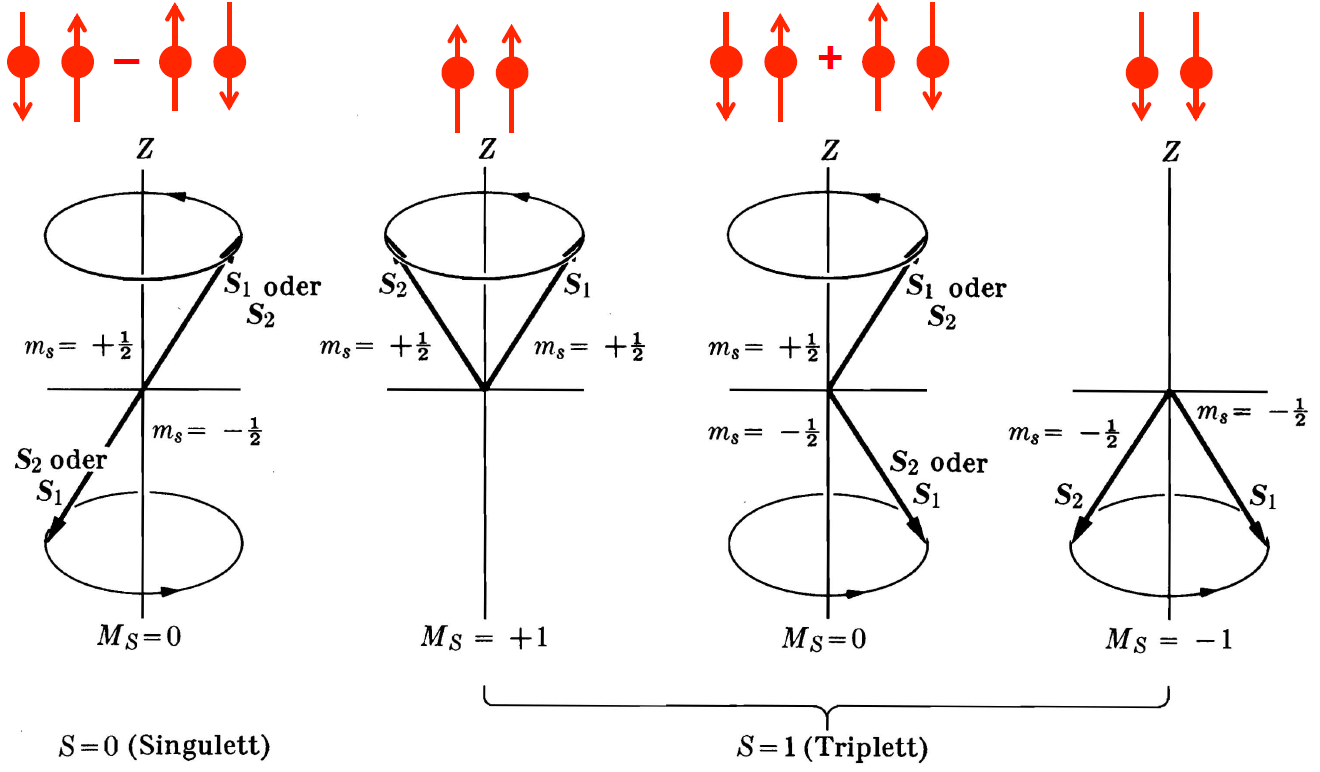
\includegraphics[width = 15cm]{ph_spin.png}\\
\end{tabular}\newpage
\begin{tabular}{p{4cm} p{15cm}}
Anzahl versch. Wellenfkt.	& Ein Zwei-Teilchen System mit je $n$ verschiedenen Zust�nden hat $\tfrac{1}{2} n(n+1)$ symmetrische und $\tfrac{1}{2} n(n-1)$ antisymmetrische Zust�nde. Dies gilt selbstverst�ndlich f�r Bahn- und Spinwellenfkt. Merke: Ein Teilchen mit Spin $S$ hat $n = 2S+1$ versch. Zust�nde\\
Ausschliessungsprinzip		& Jeder Quantenzustand $(n,l,m_l,m_s)$ kann h�chstens von einem Elektron (allg. Fermionen) eingenommen werden. Die Anzahl Zust�nde ist somit beschr�nkt durch die Abh�ngigkeiten der Quantenzahlen.\\
Regel von Hund			& Im Grundzustand von Atomen hat der resultierende Spin den gr�sstm�glichen Wert, der mit dem Ausschliessungsprinzip vereinbar ist\\
Elektronenkonfiguration		& $\text{(Hauptquantenzahl)(Bahndrehimpuls)}^{\text{Anz.Elektronen}}\quad $ Bsp: $1s^2 2s^2 2p$ 5$e^- \Rightarrow$ Bor\\
Besetzungszahl (max. \# $e^-$)	& 2(2l+1)\\
Auswahlregeln (Atom�berg�nge) 	& \begin{tabular}[t]{l}
             		  Emission und Absorption von Photonen:\\
			  $\Delta l = l_f - l_i = \pm 1$\\
			  $\Delta j = j_f - j_i = 0, \pm 1\quad j_i = 0 \Rightarrow j_f \neq 0$
             		  \end{tabular}\\
\end{tabular}

